\documentclass[../report.tex]{subfiles}

\begin{document}

\graphicspath{{img/}{../img/}}

\section{Scrum men... Ikke helt}
\label{sec:Scrum}


\paragraph{Hvad er Scrum?}
Scrum er en agil software udviklings metode, hvis hovedm�l er at kunne h�ndtere �ndringer i kravspecifikationen mens udviklingen er i gang. Indenfor godtagelse af krav�ndringer er Scrum mods�tningen til vandfaldsmodellen, som ikke tager sig p�nt i et milj� med mange krav �ndringer.

\paragraph{Scrum men... Hvad mangler s�?} I target-projektet bliver der arbejdet efter Scrum, men ikke Scrum i dets fulde forstand. I det projekt blev det besluttet at k�re l�st p� nogle af Scrums discipliner, fordi der var enighed om at det ikke gav meget mening for en projektgruppe der kun m�des et par gange om ugen.\\

\begin{figure}[H]
\centering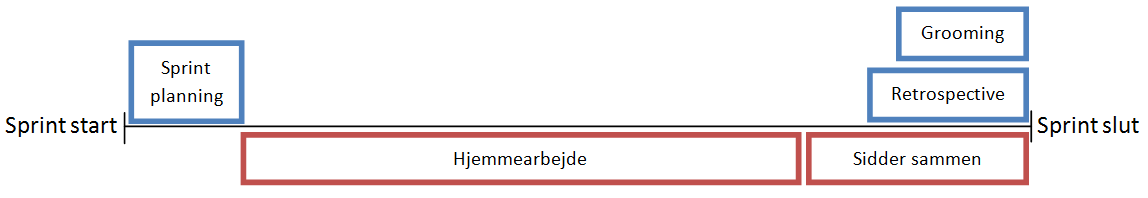
\includegraphics[scale=0.45]{SCRUMtimeLine.png}
\caption{Sprint tidslinje}
\end{figure}


\begin{tabularx}{14cm}{c|X}
\textbf{Aktiviteter}  & \textbf{�ndringer} \\
Scrum roller & I et eksamensprojekt er det urealistisk at have en person til kun at v�re product owner. I target-projektet er product owner ene og alene ansvarlig for kommunikation med stakeholders og prioritering af product items, men han er ogs� udvikler i Scrum teamet     \\ 
 & \\
Scrum Board & Scrum boardet er den centrale oversigt over hvad der skal laves og er lavet. Boardet fungerer efter vores erfaringer ogs� som stor motivationsfaktor. Da projektgruppen i target-projektet ikke har et fast lokale, er et fysisk board dog ikke muligt, s� online v�rkt�jet Trello bliver brugt i stedet\footnote{Trello.com} \\
 & \\
Standup meeting & Der blev ikke afholdt nogen standup meetings \\
 & \\
Tidstagning & Der blev i fire sprints taget tid p� arbejdet med Toggl\footnote{Toggl.com}\\
 & \\
\end{tabularx} 

\todo mere omkr. hvad vi har pr�vet

\end{document}